\documentclass[a4paper]{article}

%% Language and font encodings
\usepackage[english]{babel}
\usepackage[utf8x]{inputenc}
\usepackage[T1]{fontenc}
\usepackage[section]{placeins}
\usepackage{graphicx}
\usepackage{caption}
\usepackage{subcaption}
\usepackage{float}
\usepackage{verbatim}
\usepackage{color,soul}
\usepackage{indentfirst}



%% Sets page size and margins
\usepackage[a4paper,top=3cm,bottom=2cm,left=3cm,right=3cm,marginparwidth=1.75cm]{geometry}

%% Useful packages
\usepackage{amsmath}
\usepackage{graphicx}
\usepackage[colorinlistoftodos]{todonotes}
\usepackage[colorlinks=true, allcolors=blue]{hyperref}
\usepackage{listings}
\usepackage{color} %red, green, blue, yellow, cyan, magenta, black, white
\definecolor{mygreen}{RGB}{28,172,0} % color values Red, Green, Blue
\definecolor{mylilas}{RGB}{170,55,241}

\title{ECE 271, Example Design Project, Group 0}
\author{Matthew Shuman}
\date{May 9th, 2018}

\begin{document}

\lstset{language=Verilog,%
    basicstyle=\tiny \color{red},
    breaklines=true,%
    keywordstyle=\color{blue},%
    morekeywords=[2]{1}, keywordstyle=[2]{\color{black}},
    identifierstyle=\color{black},%
    stringstyle=\color{mylilas},
    commentstyle=\color{mygreen},%
    showstringspaces=false,%without this there will be a symbol in the places where there is a space
    numbers=left,%
    numberstyle={\tiny \color{black}},% size of the numbers
    numbersep=9pt, % this defines how far the numbers are from the text
    emph=[1]{for,end,break},emphstyle=[1]\color{red}, %some words to emphasise
    %title=\lstname
}

\maketitle
\tableofcontents
\newpage
\textbf{\textcolor{red}{\hl{This document is a template for the general formatting of the design report.  The LaTex source is provided, and will help your team create a high quality professional report. Your team may opt to use another word processor, but it will require substantial effort to produce a high quality report. }}}
\section{Project Description}
Inputs:  This design reads a VCR remote, a PS/2 Keyboard, and/or a 272 Button board.  If more than one input source is used for this project, use some of the 4 DIP switches to select which source is enabled at a given time.

Outputs:  There is one set of outputs, for the SNES console.  

\textbf{\textcolor{red}{\hl{Note that the diagram in figure 1 a good starting point for the top level diagram for the 2018 project.  }}}


\vspace{.25in}
A good top level diagram would have:
\begin{enumerate}
\item Clock oscillator (default 2.08 MHz)
\item A clock divider to make slower speeds
\item Include the input clock for necessary blocks, such as the VCR remote receiver
\end{enumerate}

\begin{figure}[h]
  \centering
    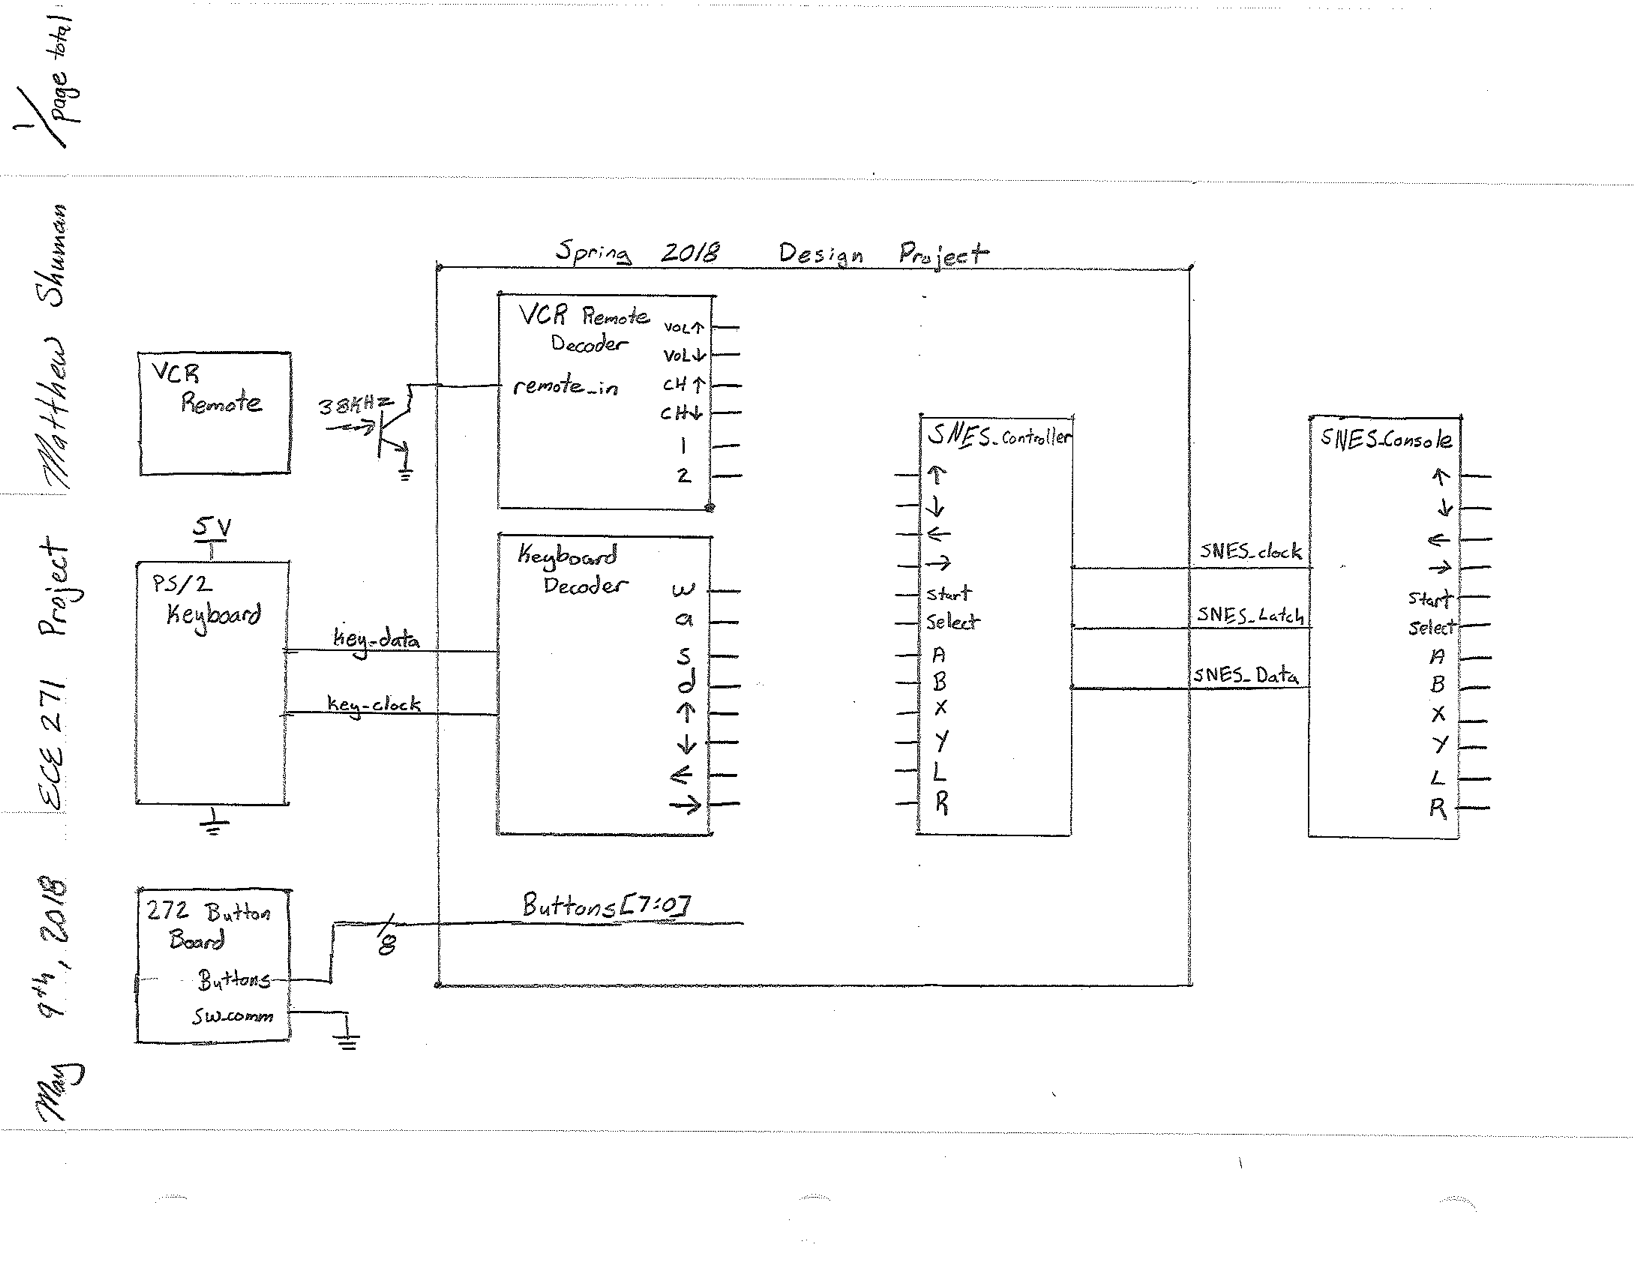
\includegraphics[width=.8\textwidth]{Images/2018Description.png}
	\caption{This image is legible, and conveys the point of the design.  Your image can be hand drawn, but it must have straight lines, use your OSU ID.  I don't recommend drafting this on the computer, because there aren't any decent tools to draw these block diagrams quickly.}
    \label{fig:2018Desc}
\end{figure}

\vspace{.25in}
The hardware diagram in figure \ref{fig:Hardware} is useful for showing the pin connections between the FPGA and hardware modules.  Good hardware diagrams have the following items:
\begin{enumerate}
\item Power and ground connections for each hardware module
\item Pin numbers being used on the FPGA
\item Descriptions of how the wires are connected, such as wire colors
\end{enumerate}

\begin{figure}[h]
  \centering
    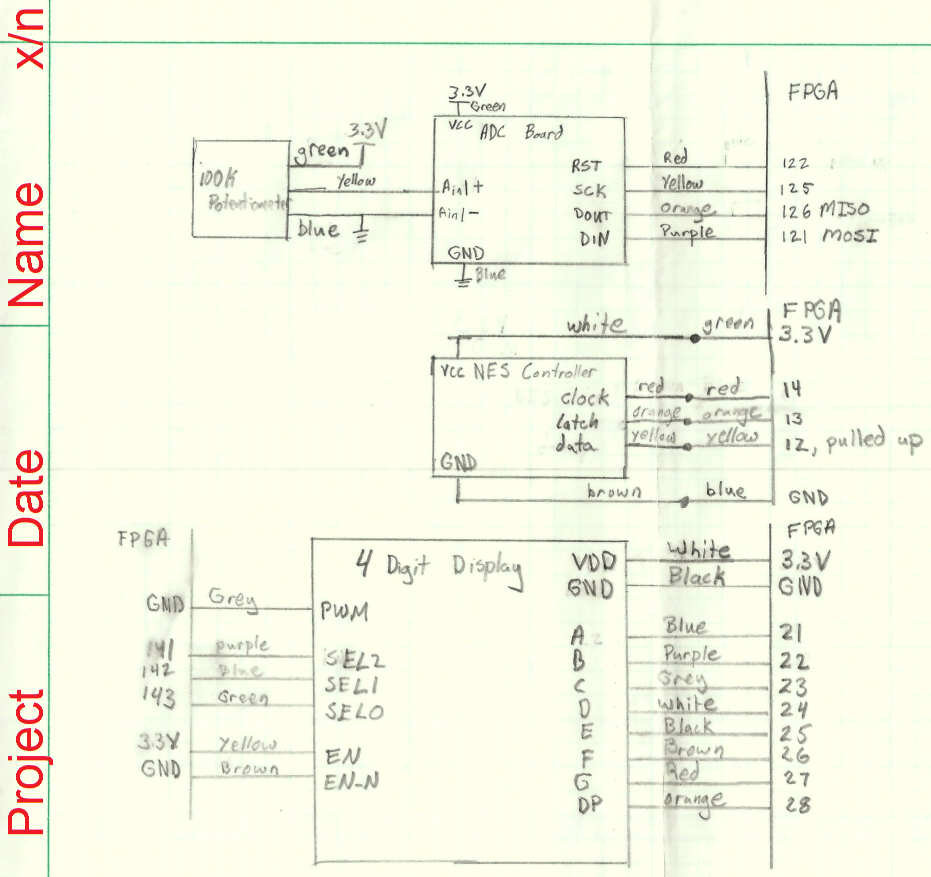
\includegraphics[width=.8\textwidth]{Images/Hardware.png}
	\caption{The hardware diagram shows which pins are used on the FPGA, module boards, and relevant supply voltages for the different pieces of hardware used in the system.}
    \label{fig:Hardware}
\end{figure}


\newpage
\section{High Level Description}
Inputs:  This reads a NES controller and the analog voltage of a potentiometer.

Outputs:  This displays a 4 digit value on a seven segment display.

\begin{figure}[h]
  \centering
    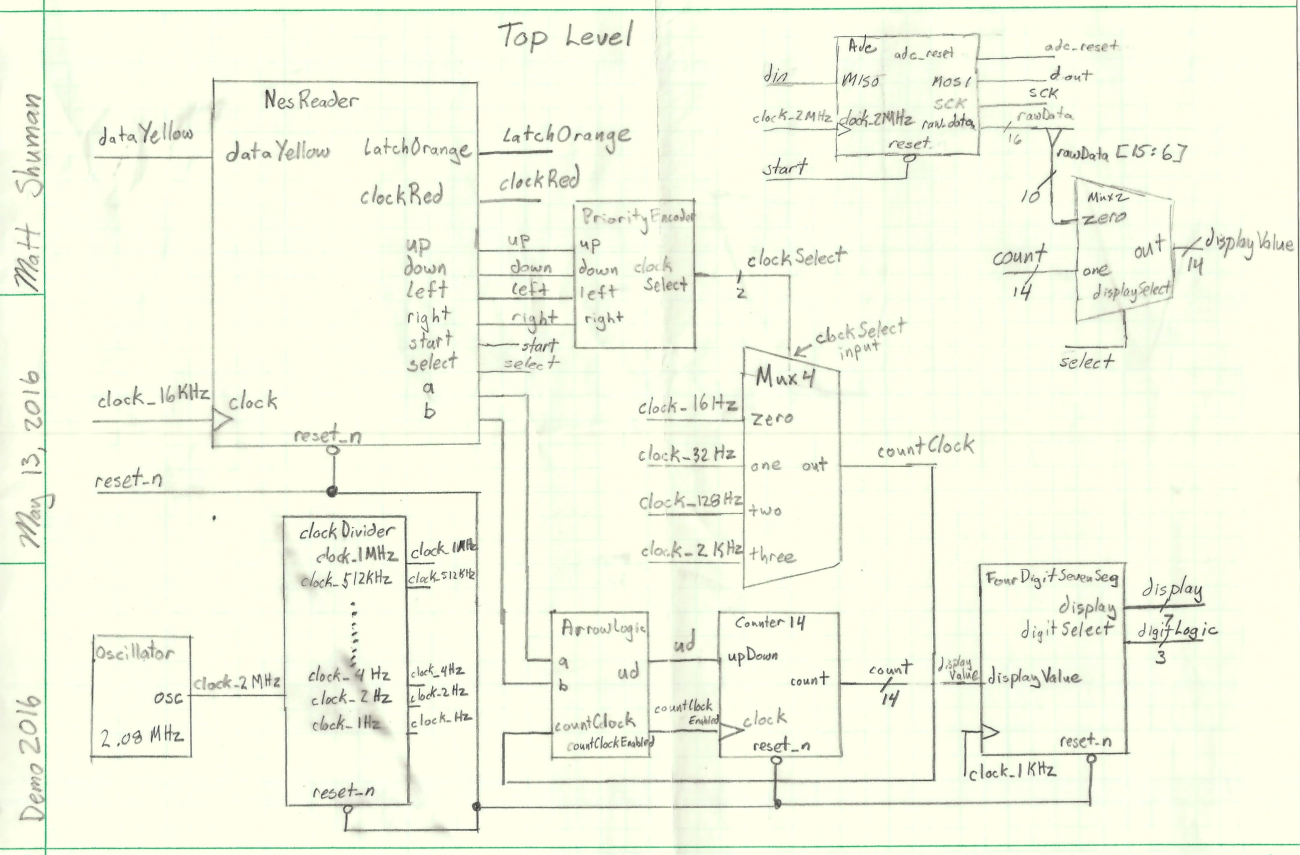
\includegraphics[width=.5\textwidth]{Images/TopLevel.png}
	\caption{The top level design for the 2016 project.  This would be improved by combining the priority encoder and Mux4 into a single clock select block.  Combining the ArrowLogic and Counter14 would also make this diagram better.  Use chapter 1 concepts wisely on this diagram, specifically hierarchy, modularity, regularity, and discipline.}
    \label{fig:TopLevelDiagram}
\end{figure}

\vspace{.25 in}

Put your simulation results for the TopLevel results here

\subsection{Functional Unit}
Inputs:  This reads a 14 bit value, uses a 1 KHz clock signal, and has an active low reset.\newline


Outputs:  display[6:0] will control which number is displayed on the seven segment display.  A 0 means that segment LED is on and a 1 means that segment LED is off.  digitSelect[2:0] controls which digit is illuminated.  The table below shows how the digitSelect operates.


\begin{center}
  \begin{tabular}{ c | l }
  \hline			
  000 & 1's digit \\
  001 & 10's digit \\
  011 & 100's digit \\
  100 & 1000's digit \\
  \hline  
  \end{tabular}
\end{center}

\begin{figure}[h]
  \centering
    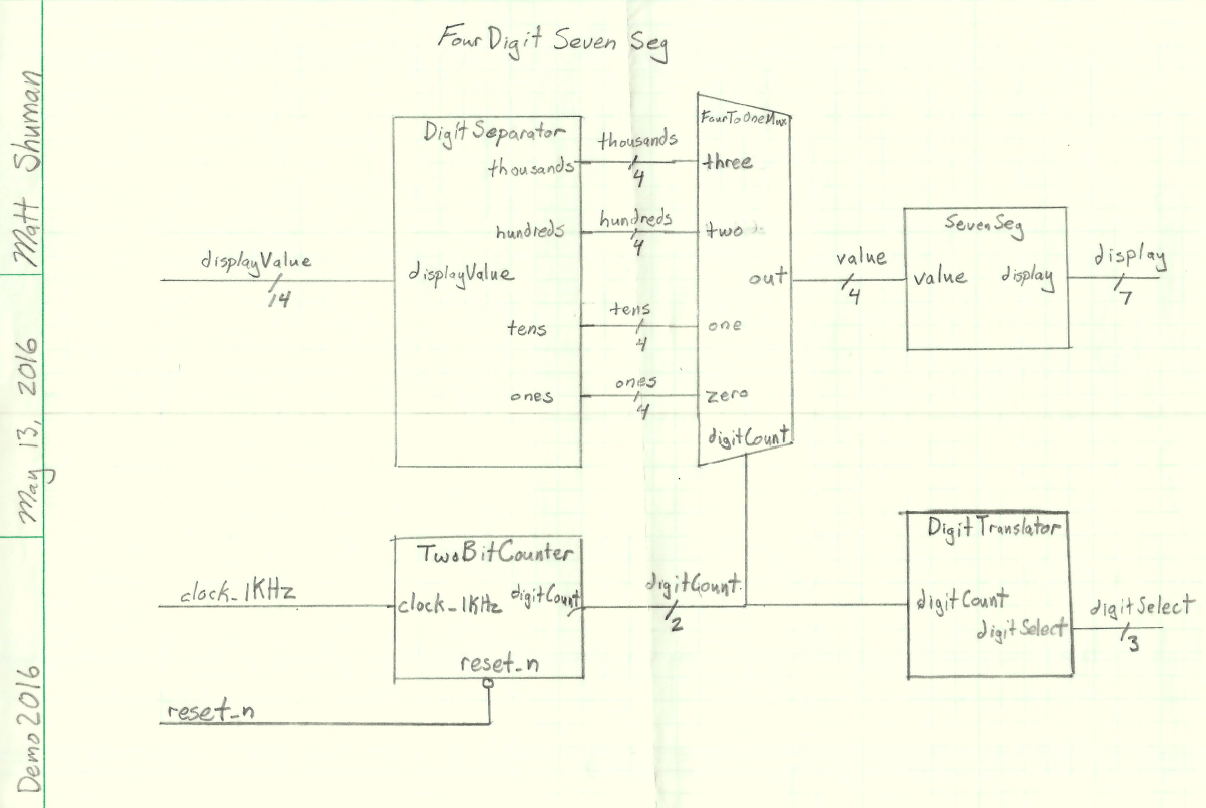
\includegraphics[width=.5\textwidth]{Images/FunctionalUnit.png}
	\caption{This is an expanded view of the block shown in the high level digram.}
    \label{fig:FourDigSevenSegment}
\end{figure}

\vspace{.25 in}
Put the simulation results for the functional unit here.

\subsubsection{Individual Block}
The individual block shown in figure \ref{fig:IndBlock} was lab 3 of the ECE 272 Lab.

Inputs:  value[3:0] ranges between 0 and 15

Outputs:  display[6:0] determines which LEDs should be on to display a number on the seven segment display.  A zero turns on the LED, a 1 turns off the LED.

\begin{figure}[h]
  \centering
    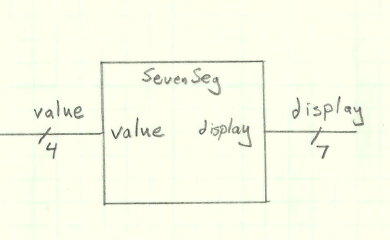
\includegraphics[width=.5\textwidth]{Images/IndividualBlock.png}
	\caption{This block was done in lab 3, by making K-Maps and drawing the logic gates needed to make this block of combinational logic.  In chapter 4 this was done in System Verilog.}
    \label{fig:IndBlock}
\end{figure}
\vspace{.25 in}
Put the simulation results for the individual blocks here.

\subsubsection{Next Individual Block}
\subsubsection{Next Individual Block}
\subsubsection{Next Individual Block}

\subsection{Next Functional Unit}
\subsubsection{Individual Block}
\subsubsection{Next Individual Block}
\subsubsection{Next Individual Block}

\subsection{Next Functional Unit}
\subsubsection{Individual Block}
\subsubsection{Next Individual Block}
\subsubsection{Next Individual Block}
\subsubsection{Next Individual Block}
\subsubsection{Next Individual Block}

\appendix
\section{SystemVerilog Files}
%Use the lst command to insert the SystemVerilog file, and comment it nicely.
\lstinputlisting{./SystemVerilog/TopLevel.v}
\subsection{Four Digit Display}
\lstinputlisting{./SystemVerilog/FourDigitSevenSeg.v}
\lstinputlisting{./SystemVerilog/DigitSeparator.v}
\lstinputlisting{./SystemVerilog/SevenSeg.v}

\section{Simulation Files (Do scripts)}
\lstinputlisting{./DoFiles/ExampleDo.do}

%\bibliographystyle{ieeetr}
%\bibliography{sample}


\end{document}